\documentclass[11pt,a4paper]{article}
\usepackage[T1]{fontenc}
\usepackage[margin=2.3cm]{geometry}
\usepackage{amsmath,amssymb}
\usepackage{graphicx}
\usepackage[dvipsnames]{xcolor}
\usepackage{enumitem}
\usepackage[colorlinks=true,linkcolor=blue,urlcolor=blue]{hyperref}
\setlength{\parskip}{0.6em}
\setlength{\parindent}{0pt}
\begin{document}

\begin{center}{\LARGE\bfseries openpipeflow}\\[0.4em]{\large Size a water pipe so the flow gets through and the pump stays cheap, in three sessions.}\\[0.2em]\small PAN IIT OSS explainer \textbullet{} higher secondary to diploma / undergraduate (levels 4-5)\end{center}

\section*{Why this exists}
Water in a pipe loses pressure as it moves, and a pump pays for that loss with electricity. This explainer builds the idea from continuity and Bernoulli to friction loss and a small looped network, using only algebra and short programs.

\section*{The end goal}
Choose a pipe size that meets flow needs within a pump budget. The end goal is to choose a pipe size that meets the flow requirement within a pump-power budget. The same reasoning, with much more care, underlies the design of water supply, irrigation and process piping.

\section*{How the three sessions build up}
\begin{enumerate}[nosep]
\item \textbf{Session 1: A narrowing pipe: speed up, pressure down} (Level 1, conceptual interactive model, 60 min).
\item \textbf{Session 2: Friction loss, Reynolds number and pump power} (Level 2, mathematical engineering model, 80 min).
\item \textbf{Session 3: A town network, solved and validated} (Level 3, simulation and validation, 90 min).
\end{enumerate}

\section{Session 1: A narrowing pipe: speed up, pressure down}

\subsection*{A. Real-world problem}
Put your thumb over the end of a garden hose and the water leaves faster. Water cannot be squeezed or lost on the way, so wherever the pipe is narrower the water must move faster. But a faster stream needs energy, and in a frictionless pipe that energy can only come from the pressure. So for steady, incompressible flow through a pipe that narrows, how do the average speed and the static pressure change? This session answers it for an idealised pipe with no friction; Session 2 adds the friction. This is general education about an idealised model, not guidance for building a real water system.

\subsection*{B. Concept and theory}
Q is the volume of water passing a cross-section each second. Because water is nearly incompressible and the flow is steady, Q is the same everywhere along the pipe. For a pipe of diameter D the area is A = pi D\textasciicircum{}2 / 4 and the average speed is v = Q / A. Halving D cuts the area to a quarter, so the speed rises four times. Bernoulli's equation says that along a level, frictionless streamline the quantity p + (1/2) rho v\textasciicircum{}2 stays constant: the term (1/2) rho v\textasciicircum{}2 is the dynamic pressure. Where v rises, the static pressure p must fall by the same amount.

\begin{itemize}[nosep]
\item Q: volume flow rate (m\textasciicircum{}3/s (1 L/s = 0.001 m\textasciicircum{}3/s))
\item D: inside diameter of the pipe (m)
\item A: cross-section area, pi D\textasciicircum{}2 / 4 (m\textasciicircum{}2)
\item v: average speed of the water (m/s)
\item p: static (gauge) pressure (Pa (1 kPa = 1000 Pa))
\item rho: density of water, 998 at 20 C (kg/m\textasciicircum{}3)
\end{itemize}

\begin{equation*}
Q = A\,v = \tfrac{\pi}{4}D^2\,v
\end{equation*}

\begin{equation*}
A_1 v_1 = A_2 v_2 \;\Rightarrow\; v_2 = v_1\left(\frac{D_1}{D_2}\right)^2
\end{equation*}

\begin{equation*}
p + \tfrac12 \rho v^2 = \text{constant} \;\Rightarrow\; p_2 = p_1 + \tfrac12 \rho\,(v_1^2 - v_2^2)
\end{equation*}

\begin{center}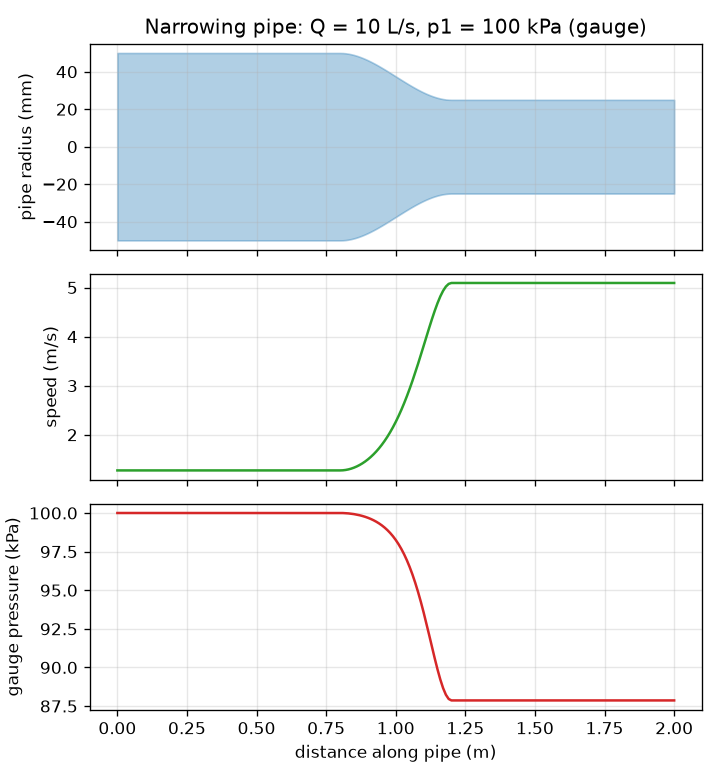
\includegraphics[width=0.85\linewidth]{figures/s01_narrowing_pipe.png}\\\small A narrowing pipe: the speed rises and the gauge pressure falls in the narrow section.\end{center}

\subsection*{E. Worked example}
Water flows at Q = 10 L/s through a 100 mm pipe at a gauge pressure of 100 kPa, then through a smooth narrowing to 50 mm. Find the speeds and the pressure in the narrow section.
\begin{enumerate}[nosep]
\item Convert: Q = 10 L/s = 0.010 m\textasciicircum{}3/s. Areas: A1 = pi (0.100)\textasciicircum{}2 / 4 = 0.007854 m\textasciicircum{}2 and A2 = pi (0.050)\textasciicircum{}2 / 4 = 0.001963 m\textasciicircum{}2.
\item Speeds: v1 = 0.010 / 0.007854 = 1.273 m/s and v2 = 0.010 / 0.001963 = 5.093 m/s. Check: (100/50)\textasciicircum{}2 = 4 and 4 x 1.273 = 5.093.
\item Dynamic pressures: (1/2)(998)(1.273)\textasciicircum{}2 = 808.9 Pa and (1/2)(998)(5.093)\textasciicircum{}2 = 12 943 Pa (about 0.81 kPa and 12.94 kPa).
\item p2 = 100 kPa + 0.81 kPa - 12.94 kPa = 87.87 kPa (gauge).
\item Sanity check: p + dynamic pressure = 100.81 kPa at both ends, and a narrower pipe gave a lower pressure, as expected.
\end{enumerate}
\textbf{Answer.} v1 = 1.273 m/s, v2 = 5.093 m/s (four times faster) and p2 = 87.87 kPa, a drop of 12.13 kPa.

\subsection*{F. Questions}
\begin{enumerate}[nosep]
\item \textbf{Conceptual.} A pipe narrows. Explain in words why the water speeds up and why its static pressure falls, and name one thing the idealised model leaves out.
\item \textbf{Numerical.} Water at 5 L/s flows at 150 kPa gauge through an 80 mm pipe that narrows to 40 mm. Find v1, v2 and p2. Check the units.
\item \textbf{Graph and simulation interpretation.} In the app, set the narrow diameter larger than the wide one (a pipe that widens). What does the pressure graph do, and is this realistic?
\item \textbf{Design and optimisation challenge.} Design: Q = 20 L/s flows at 100 kPa gauge in a 100 mm pipe. A flow-measuring throat must reach a speed of at least 5 m/s, but the gauge pressure must stay above 80 kPa. Choose a throat diameter from 50, 60, 70, 80 mm and justify it.
\end{enumerate}

\section{Session 2: Friction loss, Reynolds number and pump power}

\subsection*{A. Real-world problem}
A pump must push 20 litres of water per second through a 500 m pipe to a tank 10 m higher. A thin pipe is cheap, but the water rubs on the wall and the pump must work very hard; a fat pipe wastes less energy but costs more. How big is the friction, how much power does the pump need, and what is the smallest standard pipe that keeps the pump within a 7 kW budget? This is a simplified teaching model for sizing ideas, not a hydraulic design method; real projects need a qualified engineer, pump curves and safety factors.

\subsection*{B. Concept and theory}
Friction turns some of the water's energy into heat, so the head (energy per unit weight, written as a height in metres) falls along the pipe. The Reynolds number Re = v D / nu compares inertia with viscosity: below about 2000 the flow is smooth (laminar), above about 4000 it is turbulent. The Darcy-Weisbach equation gives the friction head loss h\_f = f (L/D) v\textasciicircum{}2 / (2 g), where f is the friction factor: exactly 64/Re when laminar, and for turbulent flow the Swamee-Jain approximation that depends on Re and on the relative roughness e/D. Bends, valves and entrances add a minor loss h\_m = K v\textasciicircum{}2 / (2 g). The pump must lift the water by the static height and also make up the losses, so H = lift + h\_f + h\_m, the water power is rho g Q H and the electric power is that divided by the efficiency eta.

\begin{itemize}[nosep]
\item Re: Reynolds number (no unit)
\item nu: kinematic viscosity (1.0e-6 for water at 20 C) (m\textasciicircum{}2/s)
\item f: Darcy friction factor (no unit)
\item e: wall roughness height (0.15 mm for an old steel pipe) (mm or m)
\item L: pipe length (m)
\item K: total minor-loss coefficient of bends and valves (no unit)
\item H: pump head (m)
\item eta: pump and motor efficiency (0.65 here) (no unit)
\item P: electric power (W (1 kW = 1000 W))
\end{itemize}

\begin{equation*}
Re = \frac{v D}{\nu}, \qquad v = \frac{4Q}{\pi D^2}
\end{equation*}

\begin{equation*}
f = \frac{64}{Re}\;(Re<2000), \qquad f = \frac{0.25}{\left[\log_{10}\!\left(\frac{e/D}{3.7} + \frac{5.74}{Re^{0.9}}\right)\right]^2}\;(Re>4000)
\end{equation*}

\begin{equation*}
h_f = f\,\frac{L}{D}\,\frac{v^2}{2g}, \qquad h_m = K\,\frac{v^2}{2g}
\end{equation*}

\begin{equation*}
H = h_{\text{lift}} + h_f + h_m, \qquad P_{\text{elec}} = \frac{\rho g Q H}{\eta}
\end{equation*}

\begin{center}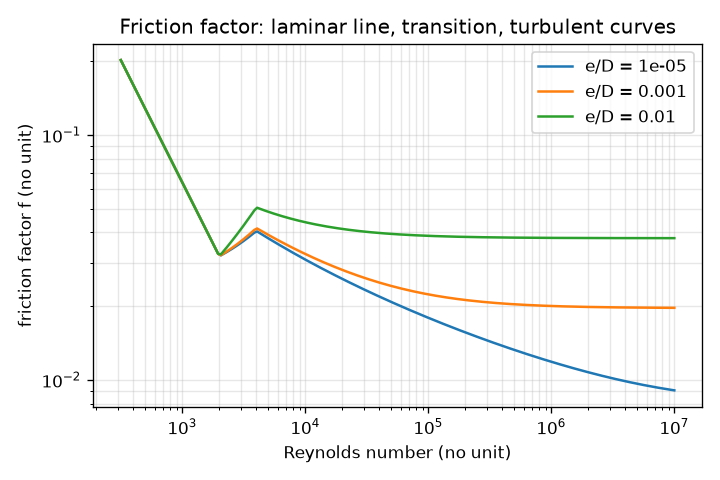
\includegraphics[width=0.85\linewidth]{figures/s02_friction_factor.png}\\\small Friction factor against Reynolds number: laminar line, transition, then turbulent curves for three roughnesses.\end{center}

\subsection*{E. Worked example}
Water at 20 L/s goes through 500 m of 125 mm pipe (roughness 0.15 mm, K = 5) to a tank 10 m higher. The pump and motor are 65 percent efficient. Find the electric power.
\begin{enumerate}[nosep]
\item Q = 0.020 m\textasciicircum{}3/s, D = 0.125 m. v = 4(0.020) / (pi (0.125)\textasciicircum{}2) = 1.630 m/s. Velocity head v\textasciicircum{}2 / (2 g) = 2.656 / 19.62 = 0.1354 m.
\item Re = v D / nu = 1.630 x 0.125 / 1.0e-6 = 203 700, which is turbulent. Relative roughness e/D = 0.00015 / 0.125 = 0.0012.
\item Swamee-Jain: log10(0.0012 / 3.7 + 5.74 / 203 700\textasciicircum{}0.9) = log10(0.000324 + 0.0000957) = -3.3768, squared 11.402, so f = 0.25 / 11.402 = 0.0219 (the code gives 0.02193).
\item Friction loss h\_f = 0.0219 x (500 / 0.125) x 0.1354 = 11.87 m. Minor loss h\_m = 5 x 0.1354 = 0.68 m.
\item Pump head H = 10 + 11.87 + 0.68 = 22.55 m. Water power = 998 x 9.81 x 0.020 x 22.55 = 4415 W.
\item Electric power = 4415 / 0.65 = 6793 W, about 6.79 kW: just inside the 7 kW budget. Speed 1.63 m/s is below 3 m/s.
\end{enumerate}
\textbf{Answer.} v = 1.63 m/s, Re = 203 700, f = 0.0219, h\_f = 11.87 m, h\_m = 0.68 m, H = 22.55 m, electric power 6.79 kW. The next smaller standard size, 100 mm, needs 14.8 kW, so 125 mm is the smallest that fits 7 kW.

\subsection*{F. Questions}
\begin{enumerate}[nosep]
\item \textbf{Conceptual.} Why does doubling the pipe diameter reduce the friction loss by much more than a factor of two for the same flow rate?
\item \textbf{Numerical.} 12 L/s of water flows through 200 m of 100 mm pipe of roughness 0.15 mm. Find the speed, Reynolds number, friction factor, head loss and the power lost to friction (no minor losses).
\item \textbf{Graph and simulation interpretation.} Read the power-against-diameter curve for 20 L/s, 500 m, 10 m lift. About what power is needed at 100 mm, 125 mm and 200 mm, and what limits the curve for large diameters?
\item \textbf{Design and optimisation challenge.} Design: the same job (20 L/s, 500 m, 10 m lift, K = 5, roughness 0.15 mm, 65 percent efficient) but a smaller budget of 5 kW. Choose a standard size from 100, 125, 150, 200 mm. What if the budget were 4 kW? Justify with speed and trade-offs.
\end{enumerate}

\section{Session 3: A town network, solved and validated}

\subsection*{A. Real-world problem}
A town is fed from a tank on a hill. Pipes branch and close into a loop, and each street takes some water. No formula gives the flow in each pipe; it must be found numerically. And a number from a program is worth nothing until it has been checked. Can you solve a small looped network, prove the answer is right, and see which pipe sizes keep every node above 20 m of pressure head? This is a simplified teaching model, not a hydraulic design tool: real networks need hydraulic modelling software, peak-demand analysis, fire flows and regulation.

\subsection*{B. Concept and theory}
A network obeys two laws. Continuity: at every node the flow in equals the flow out plus the demand. Energy: around every closed loop the head losses add to zero, because water cannot gain energy by going round in a circle. The head loss of each pipe depends on its own flow through Darcy-Weisbach, so the equations are not linear. Hardy Cross starts with flows that obey continuity, then adds a correction x to the loop flow: we need F(x) = h2 + h4 - h3 = 0, and Newton's method gives x\_new = x - F / F', where F' is the sum of the slopes dh/dQ of the loop pipes. Once the flows are known, the heads follow by subtracting the pipe losses from the tank level, and pressure head is head minus street level.

\begin{itemize}[nosep]
\item Q\_i: flow in pipe i (negative if it runs against the arrow) (m\textasciicircum{}3/s)
\item x: flow in the cross pipe B to C, the loop unknown (m\textasciicircum{}3/s)
\item h\_i: signed head loss of pipe i (m)
\item H: hydraulic head at a node (m)
\item z: street level at a node (m)
\item pressure head: H - z (m of water (1 m = 9.79 kPa))
\item F: head-loss imbalance around the loop (m)
\end{itemize}

\begin{equation*}
\sum Q_{\text{in}} - \sum Q_{\text{out}} - q_{\text{demand}} = 0 \quad\text{(each node)}
\end{equation*}

\begin{equation*}
F(x) = h_2(Q_2) + h_4(x) - h_3(Q_3) = 0, \qquad Q_2 = q_B + x,\; Q_3 = q_C - x
\end{equation*}

\begin{equation*}
x_{k+1} = x_k - \frac{F(x_k)}{\sum_i \mathrm{d}h_i/\mathrm{d}Q_i}
\end{equation*}

\begin{equation*}
H_A = H_T - h_1, \quad H_B = H_A - h_2, \quad H_C = H_A - h_3, \quad \text{pressure head} = H - z
\end{equation*}

\begin{center}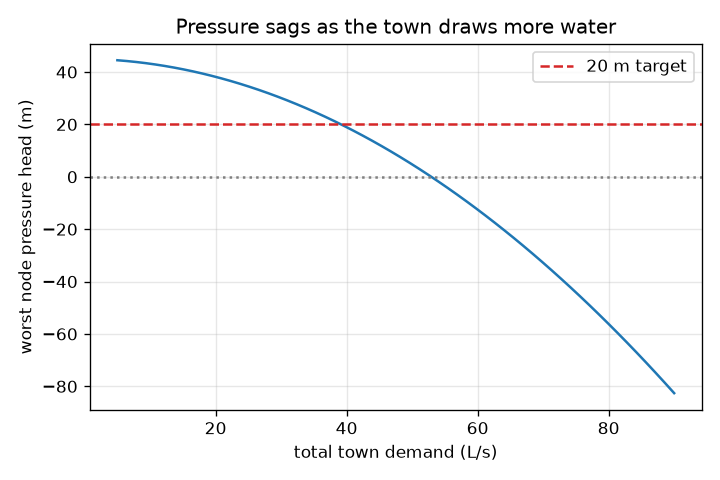
\includegraphics[width=0.85\linewidth]{figures/s03_pressure_vs_demand.png}\\\small Worst node pressure head against total demand; the dashed line is the 20 m target.\end{center}

\subsection*{E. Worked example}
The tank (level 70 m) feeds node A through a 1200 m, 200 mm main (roughness 0.15 mm). Pipes 2, 3 and 4 are 125 mm. The town takes 30 L/s (18 L/s at B, 12 L/s at C). Find the main-pipe loss and the pressure head at A by hand, then check the numerical flows and pressure at the other nodes.
\begin{enumerate}[nosep]
\item Main pipe: Q = 0.030 m\textasciicircum{}3/s, D = 0.200 m, v = 4(0.030) / (pi (0.2)\textasciicircum{}2) = 0.955 m/s, v\textasciicircum{}2 / (2 g) = 0.04648 m.
\item Re = 0.955 x 0.2 / 1.0e-6 = 190 986 and e/D = 0.00075, so Swamee-Jain gives f = 0.02021.
\item h1 = f (L/D) v\textasciicircum{}2 / (2 g) = 0.02021 x (1200 / 0.2) x 0.04648 = 5.64 m.
\item Head at A = 70 - 5.64 = 64.36 m; street level 20 m, so the pressure head at A is 44.36 m (about 434 kPa).
\item The program's Hardy Cross finds the loop flow in 4 iterations: Q2 = 16.17, Q3 = 13.83 and Q4 = -1.83 L/s (the cross pipe runs from C to B). Losses are 9.42 m, 9.29 m and -0.13 m.
\item Checks: at node B the inflow is 16.17 + 1.83 = 18.00 L/s, equal to its demand; round the loop 9.42 - 0.13 - 9.29 = 0.00. Pressure heads: B = 39.94 m and C = 30.07 m, so the worst node is C.
\end{enumerate}
\textbf{Answer.} Main pipe loss 5.64 m, pressure head at A 44.36 m; flows 30.00, 16.17, 13.83 and -1.83 L/s; pressure heads B 39.94 m and C 30.07 m. Every node is above the 20 m target and mass is conserved to 1e-12 m\textasciicircum{}3/s.

\subsection*{F. Questions}
\begin{enumerate}[nosep]
\item \textbf{Conceptual.} Why must the head losses around a closed loop add up to zero, and what does the sign of the flow in the cross pipe (pipe 4) tell you?
\item \textbf{Numerical.} For the default network at 30 L/s, the flow in pipe 3 is 13.83 L/s and in pipe 2 is 16.17 L/s. Check the continuity at node A and find the speed in pipe 3 (125 mm).
\item \textbf{Graph and simulation interpretation.} In the pressure-against-demand graph, where does the worst node pressure cross the 20 m target with the default pipes, and what does the shape of the curve say?
\item \textbf{Design and optimisation challenge.} Design: the town must serve 50 L/s with every node at 20 m or more. With 200 mm main and 125 mm branches, does it work? Choose a main from 200, 220, 250 mm and a branch from 125, 150 mm and justify.
\end{enumerate}

\section{Real-world mini-project}
\textbf{Size the pipe run for a water tank on a hill.} A village wants a pump at a stream to fill a tank on a hill 45 m higher. The pipe run is 900 m long, the fittings add a total loss coefficient K = 3, the tank must be refilled at 15 L/s and the pump plus motor is 65 percent efficient. The pump supply allows at most 12 kW electric. Use \texttt{pipe\_run\_power} from Session 3 with the standard sizes 50, 65, 80, 100, 125, 150 and 200 mm (wall roughness 0.15 mm).

\section{The path ahead}
\begin{enumerate}[nosep]
\item \textbf{Session 4: Colebrook-White friction factor.} A friction factor function that replaces the Swamee-Jain formula inside the network solver.
\item \textbf{Session 5: A general network solver.} A solver that reads any list of pipes, nodes and demands.
\item \textbf{Session 6: Pumps and tanks as network parts.} A pump element with a head-flow curve added to the network.
\item \textbf{Session 7: A day of demand.} A 24-hour simulation with a demand pattern and a tank level.
\item \textbf{Session 8: Draw the town.} A map with moving flow dots and node colours.
\end{enumerate}

\section{Answers and hints}

\subsection*{Session 1}
\begin{enumerate}[nosep]
\item \textbf{Conceptual.} Hint: Think about how much water must pass each second, and where the extra kinetic energy comes from. Solution: The same volume per second must pass every cross-section, so through a smaller area the water must move faster (A1 v1 = A2 v2). Faster water has more kinetic energy per kilogram; with no friction and no pump that energy can only come from the pressure energy, so p falls. The model leaves out friction (a real pressure also falls because of friction), turbulence and the speed differences across the cross-section.
\item \textbf{Numerical.} Hint: Convert 5 L/s to m\textasciicircum{}3/s first. Use v = 4 Q / (pi D\textasciicircum{}2), then p2 = p1 + (1/2) rho (v1\textasciicircum{}2 - v2\textasciicircum{}2). Solution: Q = 0.005 m\textasciicircum{}3/s. v1 = 4(0.005) / (pi (0.080)\textasciicircum{}2) = 0.995 m/s. v2 = 4(0.005) / (pi (0.040)\textasciicircum{}2) = 3.979 m/s (four times, since the diameter halved). p2 = 150 kPa + (1/2)(998)(0.990 - 15.83) Pa = 150 - 7.41 = 142.59 kPa. Units: m/s for speed; kg/m\textasciicircum{}3 x m\textasciicircum{}2/s\textasciicircum{}2 = Pa for pressure terms. Sanity check: the narrow section has the lower pressure.
\item \textbf{Graph and simulation interpretation.} Hint: Compare v2 with v1 and use p2 = p1 + (1/2) rho (v1\textasciicircum{}2 - v2\textasciicircum{}2). Solution: The speed falls, so the pressure curve rises above its starting value (for 100 mm widening to 150 mm at 10 L/s it goes from 100 kPa to 100.65 kPa). This is Bernoulli's pressure recovery. In a real pipe a sudden or steep widening makes the flow separate and swirl, so much of the recovery is lost; the ideal curve is the best case.
\item \textbf{Design and optimisation challenge.} Hint: Compute v and p for each diameter; the speed condition wants a small D, the pressure condition a large D. Solution: v1 = 2.546 m/s. For 70 mm: v = 5.197 m/s and p = 100 + (1/2)(998)(6.485 - 27.01)/1000 = 89.76 kPa: both conditions met. For 80 mm: v = 3.98 m/s, too slow. For 60 mm: v = 7.07 m/s and p = 100 + 499(6.485 - 49.97)/1000 = 78.3 kPa, which is below 80 kPa. For 50 mm: 10.19 m/s and about 51 kPa. So 70 mm is the only choice that works. Trade-off: a narrower throat gives a bigger, easier to read signal but wastes more pressure in real flow.
\end{enumerate}

\subsection*{Session 2}
\begin{enumerate}[nosep]
\item \textbf{Conceptual.} Hint: Count how D enters through v and through the factor L/D. Solution: For fixed Q the speed is v = 4Q / (pi D\textasciicircum{}2), so v\textasciicircum{}2 goes as 1/D\textasciicircum{}4, and the loss h\_f = f (L/D) v\textasciicircum{}2 / (2 g) has another 1/D, giving about 1/D\textasciicircum{}5 (f also changes a little). Doubling D therefore cuts the loss by about 2\textasciicircum{}5 = 32 times (the code gives 34.8 times between 100 mm and 200 mm because f changes). That is why a slightly larger pipe saves a lot of pumping power.
\item \textbf{Numerical.} Hint: v = 4Q / (pi D\textasciicircum{}2), then Re, then e/D = 0.0015 for Swamee-Jain, then h\_f, then rho g Q h\_f. Solution: v = 4(0.012) / (pi (0.1)\textasciicircum{}2) = 1.528 m/s; v\textasciicircum{}2 / (2 g) = 0.119 m. Re = 1.528 x 0.1 / 1.0e-6 = 152 800 (turbulent). f = 0.0233. h\_f = 0.0233 x (200 / 0.1) x 0.119 = 5.54 m. Power lost = 998 x 9.81 x 0.012 x 5.54 = 651 W. Units: m/s, no unit, no unit, m, W. Sanity check: the speed is moderate and the loss of 2.8 m per 100 m is plausible for a pipe of this size.
\item \textbf{Graph and simulation interpretation.} Hint: Use the app: set each diameter and read the electric power. Solution: At 100 mm about 14.8 kW, at 125 mm 6.79 kW and at 200 mm 3.37 kW. For very large pipes the friction vanishes and the power approaches the lift term alone: rho g Q (10 + small minor loss) / 0.65 = 3.0 kW. Extra diameter then buys almost nothing, while the pipe cost keeps rising. The best size is therefore where the curve first meets the budget, not the largest pipe.
\item \textbf{Design and optimisation challenge.} Hint: Use smallest\_diameter(budget, ...) or the power numbers 14.8, 6.79, 4.51 and 3.37 kW. Solution: 5 kW: 125 mm needs 6.79 kW (too much), 150 mm needs 4.51 kW (fits), so choose 150 mm with speed 1.13 m/s. 4 kW: 150 mm fails, 200 mm needs 3.37 kW and fits, speed 0.64 m/s. Trade-off: each step up in size costs more for the pipe and trench but saves running cost; a low speed also reduces noise and water hammer. Assumptions: constant 65 percent efficiency and clean water; a real design adds a margin and pump curves.
\end{enumerate}

\subsection*{Session 3}
\begin{enumerate}[nosep]
\item \textbf{Conceptual.} Hint: Think of walking around a loop and returning to the same node. Solution: The head at a node is a single number. Walking round a loop and returning to the start, the sum of the head drops (taking each in the direction of travel) must be zero, otherwise the node would have two different heads. A negative flow in pipe 4 means the water actually runs from C to B, against the arrow drawn from B to C: the shorter, bigger route through pipe 3 is carrying part of B's demand.
\item \textbf{Numerical.} Hint: Node A: flow in from pipe 1 equals the sum of flows out in pipes 2 and 3. Speed = 4 Q / (pi D\textasciicircum{}2). Solution: Out of A: 16.17 + 13.83 = 30.00 L/s, equal to the 30.00 L/s that the main delivers: balance zero. Speed in pipe 3: v = 4(0.01383) / (pi (0.125)\textasciicircum{}2) = 1.127 m/s. Units: L/s converted to m\textasciicircum{}3/s by dividing by 1000. Sanity check: speeds around 1 m/s are typical for town mains.
\item \textbf{Graph and simulation interpretation.} Hint: Use the app with the default pipes and change the total demand slider. Solution: At 30 L/s the worst pressure head is 30.07 m; at 36 L/s it is 23.8 m; at 40 L/s 18.9 m, so the crossing is a little below 40 L/s (about 39 L/s). The curve bends downward faster at higher demand because the friction loss grows roughly with the square of the flow. A small increase in demand near the limit therefore costs more pressure than the same increase at low demand. Below zero the pressure head is not physical for a real supply.
\item \textbf{Design and optimisation challenge.} Hint: Use min\_pressure\_head(d\_main=..., d\_branch=..., total\_lps=50). Solution: 200/125: worst pressure is 4.7 m at C, which fails. 250/125 gives 15.0 m, still failing: the branches are the bottleneck. 200/150 gives 20.0 m, only just. 220/150 gives 25.9 m and 250/150 gives 30.3 m. Choose the 220 mm main with 150 mm branches: it meets the target with a margin and keeps the main speed at 1.32 m/s. Trade-off: pipe cost grows with diameter, so we stop at the smallest sizes that pass with a margin; a real design would also check peak hours, fire flow and ageing.
\end{enumerate}

\section{How to join}
Read \texttt{CONTRIBUTING.md} in the repository, then pick an issue labelled \texttt{good first issue}. Repository: \url{https://github.com/KrunalPanchal1995/openpipeflow}

\end{document}
